\documentclass[11pt]{article}
\usepackage[a4paper]{geometry}


\usepackage{pgf-pie} 
\usepackage{tikz}
\usepackage{pgfplots}
\pgfplotsset{
width=7cm,
compat=1.3,
colormap name=blackwhite
%,bar cycle list name=black white
}

%\definecolor{BoxCol}{rgb}{0.9,0.9,1}
\definecolor{EMMT}{HTML}{009933}
\definecolor{CoSMaT}{HTML}{33CC33}
\colorlet{SMT}{pink!33}
\colorlet{CSMT}{orange!33}
\colorlet{CMT}{red!66}
\colorlet{WMT}{green!33}

\definecolor{Posteditor1}{HTML}{EFDECD}
%\definecolor{Posteditor2}{HTML}{FFBF00}
\definecolor{Posteditor2}{HTML}{F0DC82}
%\definecolor{Posteditor3}{HTML}{9966CC}
\definecolor{Posteditor3}{HTML}{BF94E4}
\definecolor{Posteditor4}{HTML}{CD9575}
%\definecolor{Posteditor5}{HTML}{0000FF}
%\definecolor{Posteditor5}{HTML}{FFC1CC}
%\definecolor{Posteditor5}{HTML}{ED872D}
\definecolor{Posteditor5}{HTML}{FFA700}
\definecolor{Posteditor6}{HTML}{7FFFD0}
\definecolor{Posteditor7}{HTML}{A1CAF1}
\definecolor{Posteditor8}{HTML}{ACE5EE}


\title{WMT 2015 Survey Results}
\author{}
\date{}

  \begin{document}
  
  \maketitle

\section*{Percentage of $1^{st}$ choice votes for conference acronyms}
%\begin{figure}[!h]
\begin{center}
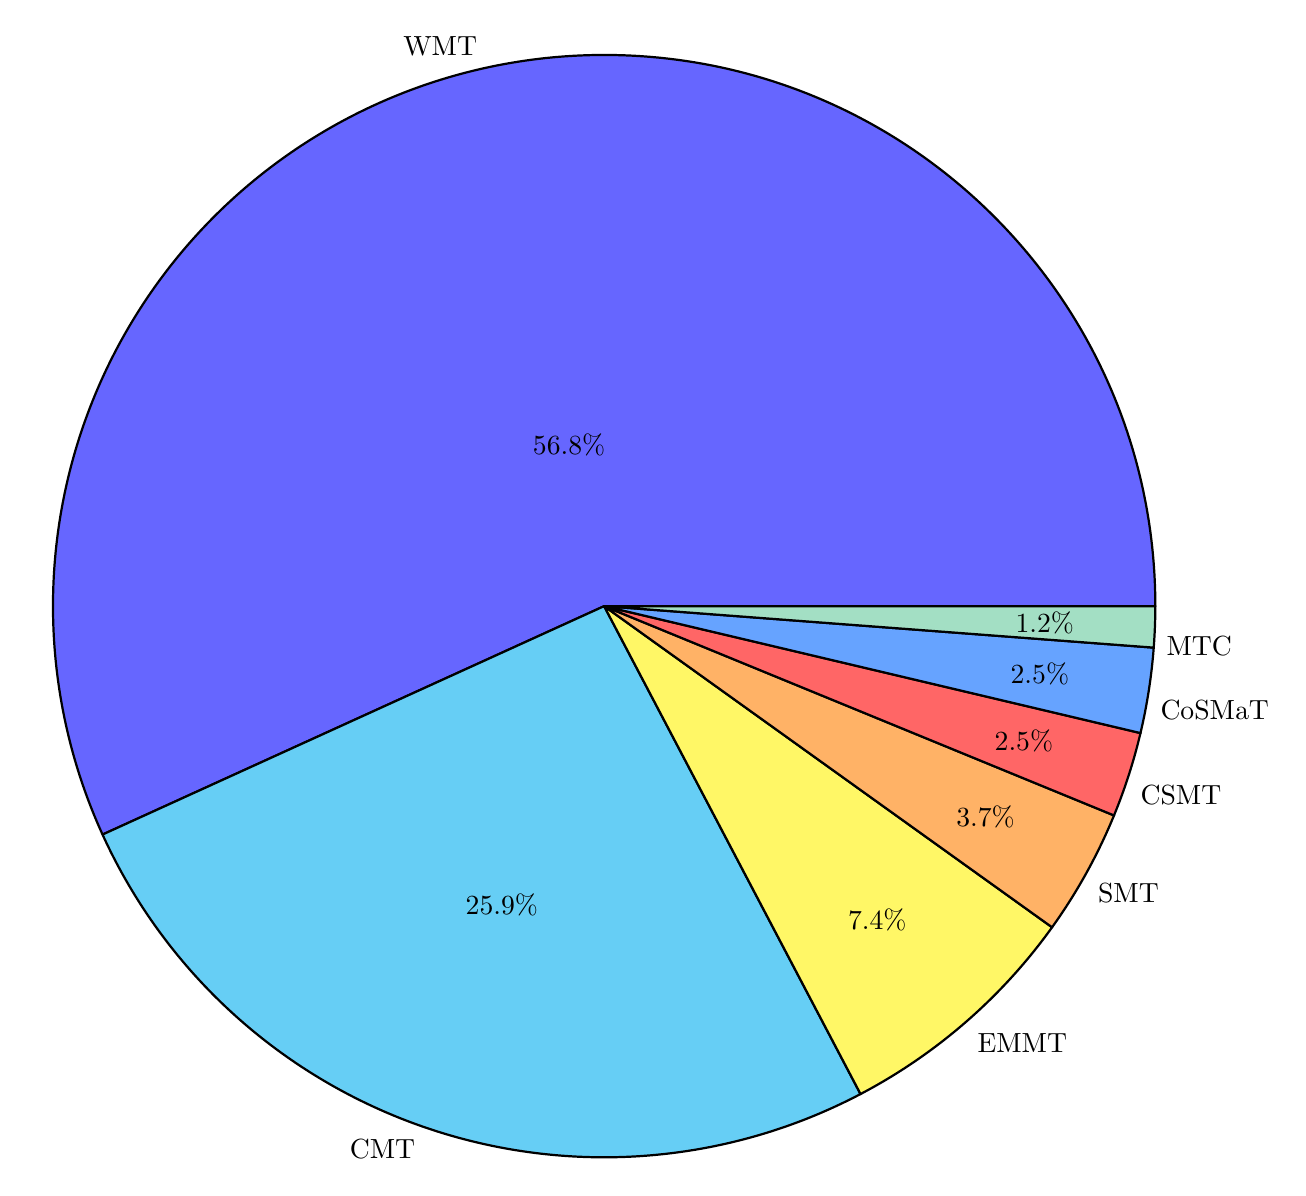
\begin{tikzpicture}
  \pie[
  	sum=auto, 
	after number=\%, 
	explode=0, 
	radius=7,
	%color={WMT, CMT, CSMT, SMT, CoSMaT, EMMT, MTC}
       ]{56.8/WMT, 25.9/CMT, 7.4/EMMT, 3.7/SMT, 2.5/CSMT, 2.5/CoSMaT,  1.2/MTC}
\end{tikzpicture}
\end{center}
%\caption{Percentage of $1^{st}$ choice votes for conference acronyms.}
%\end{figure}

\section*{Number of $1^{st}$ place votes for each name/acronym choice}
% \begin{figure}
\begin{center}
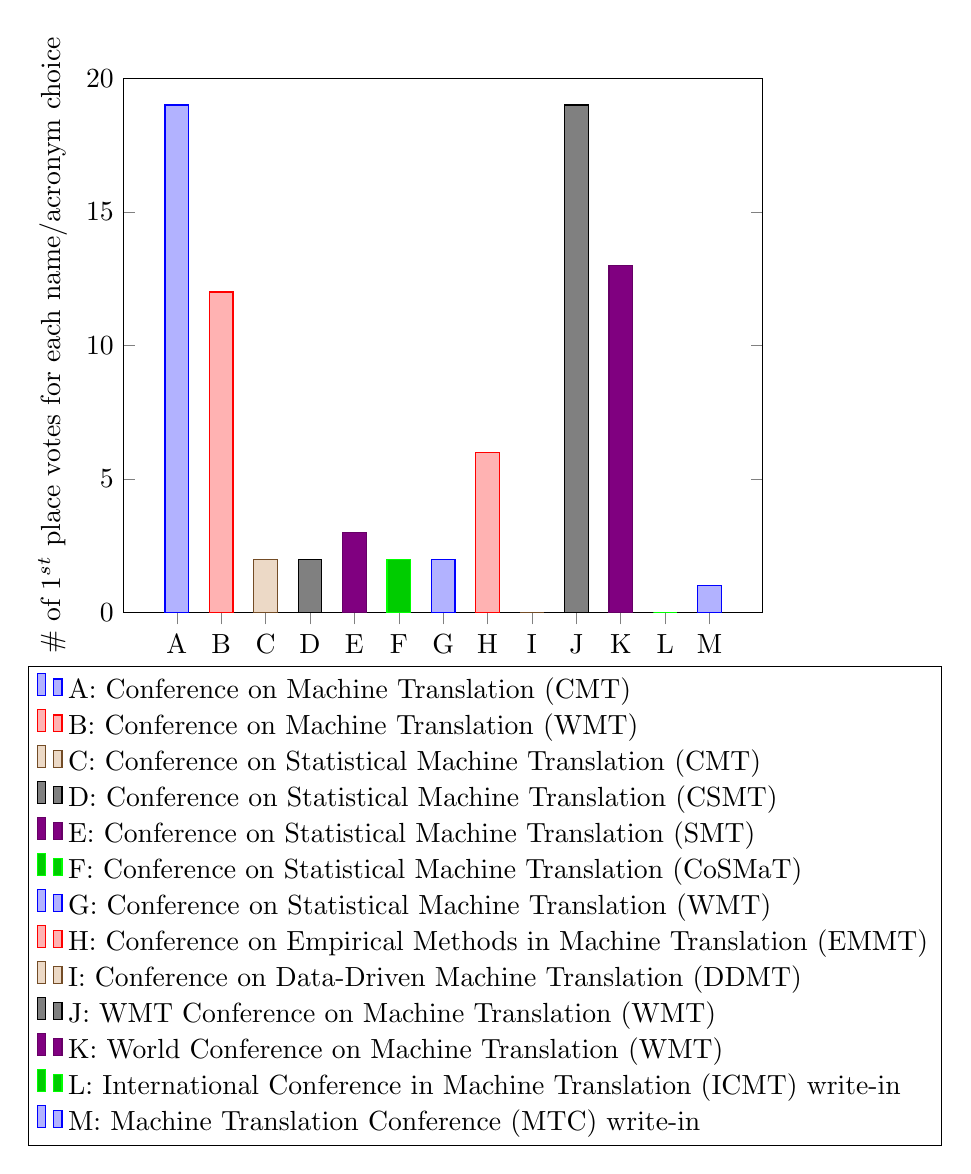
\begin{tikzpicture}
\begin{axis}[
%xmode=log,
xmode=normal,
ymode=normal,
xtick pos=left,
%xtick=data,
%ytick=data,
%ytick={45,56,63,68,72,100},
%log basis x=2,
%xticklabels={8,16,32,64,128,256,512},
%ytick={160,150,140,130,120,110,100,90,80,70,60,50,40,30,20,10},
xtick={1,2,3,4,5,6,7,8,9,10,11,12,13},
xticklabels={A,B,C,D,E,F,G,H,I,J,K,L,M},
%ytick={100,90,80,70,60,50,40,30,20,10},
%tick label style={font=\tiny},
%xlabel=Posteditor,
ylabel near ticks,
ylabel={\# of $1^{st}$ place votes for each name/acronym choice},
ymin=0,
ymax=20,
%xmin=-1,
%xmax=12,
%enlarge x limits=0.5,
%scale only axis=false,
%axis equal=false,
legend style={at={(-0.15,-0.1)},anchor=north west},
legend cell align=left,
%legend pos=outer north east,
%legend style={
%	at={(100.5,-10.15)},
%	anchor=north,
	%legend columns=-1
%},
%ybar=0pt,
width=0.8\linewidth,
%height=17cm,
ybar,
bar shift=0pt,
bar width=3mm,
%legend style={draw=none},
%legend pos=north east,
%cycle list name=exotic,
%cycle list={
%	fill=Posteditor1,
%	fill=Posteditor2,
%	fill=Posteditor3,
%	fill=Posteditor4,
%	fill=Posteditor5,
%	fill=Posteditor6,
%	fill=Posteditor7,
%	fill=Posteditor8
%	}
%bar shift=3pt
%ybar interval=0.7
]
%
%\addlegendimage{empty legend}
%\addlegendimage{area legend}\addlegendentry{TEST}  
\legend{
{A: Conference on Machine Translation (CMT)},
{B: Conference on Machine Translation (WMT)},
{C: Conference on Statistical Machine Translation (CMT)},
{D: Conference on Statistical Machine Translation (CSMT)},
{E: Conference on Statistical Machine Translation (SMT)},
{F: Conference on Statistical Machine Translation (CoSMaT)},
{G: Conference on Statistical Machine Translation (WMT)},
{H: Conference on Empirical Methods in Machine Translation (EMMT)},
{I: Conference on Data-Driven Machine Translation (DDMT)},
{J: WMT Conference on Machine Translation (WMT)},
{K: World Conference on Machine Translation (WMT)},
{L: International Conference in Machine Translation (ICMT) write-in},
{M: Machine Translation Conference (MTC) write-in}
};
\addplot coordinates{ (1,19) };
\addplot coordinates{ (2,12) };
\addplot coordinates{ (3,2) };
\addplot coordinates{ (4,2) };
\addplot coordinates{ (5,3) };
\addplot coordinates{ (6,2) };
\addplot coordinates{ (7,2) };
\addplot coordinates{ (8,6) };
\addplot coordinates{ (9,0) };
\addplot coordinates{ (10,19) };
\addplot coordinates{ (11,13) };
\addplot coordinates{ (12,0) };
\addplot coordinates{ (13,1) };
%\draw[dashed,color=black] (axis cs:0,63.8) -- (axis cs:100,63.8);
%
\end{axis}
\end{tikzpicture}
%\caption{Number of $1^{st}$ place votes for each name/acronym choice}
\end{center}
%\end{figure}
\clearpage


\section*{Total number votes for each name/acronym choice}

In the chart below, all votes for each choice are counted, not just $1^{st}$ place votes.

%\begin{figure*}
\begin{center}
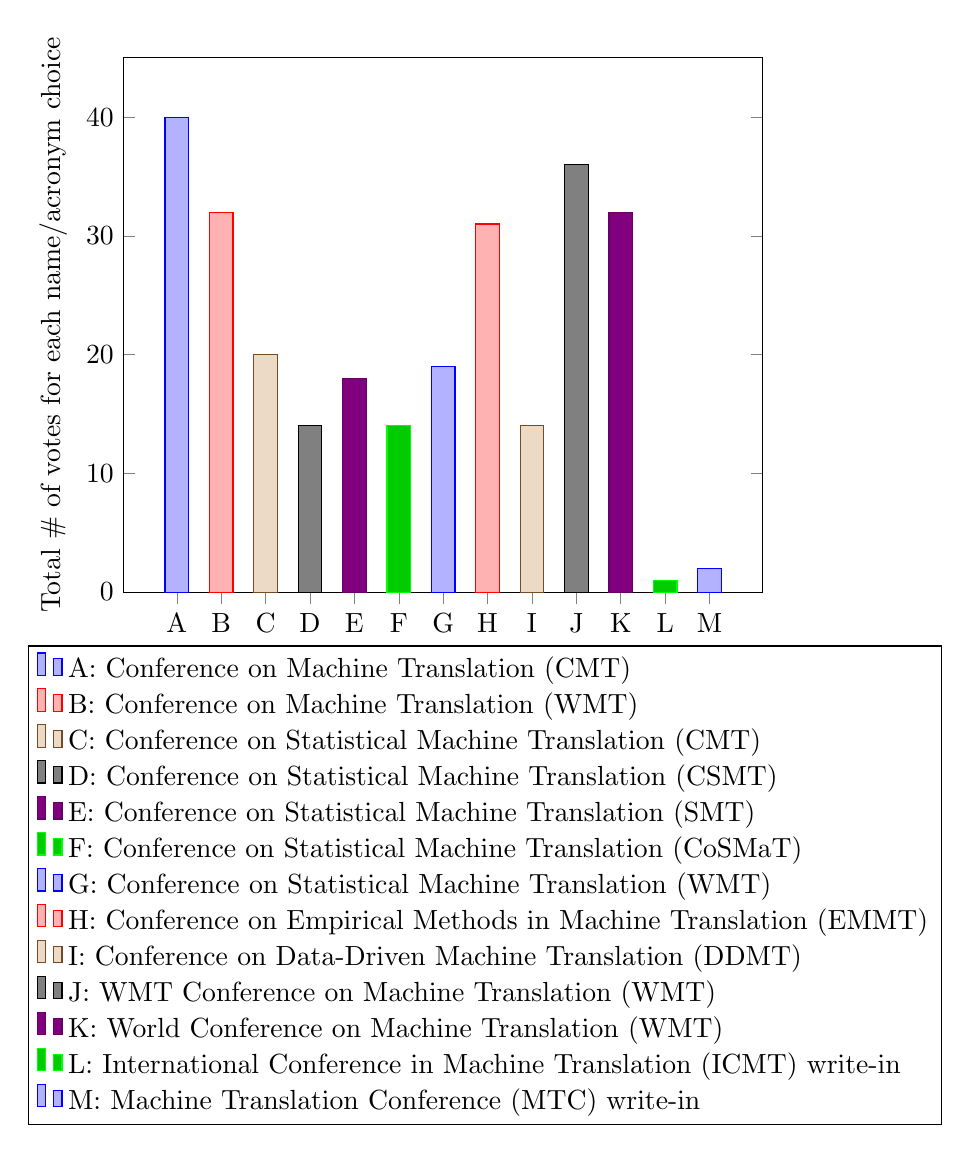
\begin{tikzpicture}
\begin{axis}[
xmode=normal,
ymode=normal,
xtick pos=left,
xtick={1,2,3,4,5,6,7,8,9,10,11,12,13},
xticklabels={A,B,C,D,E,F,G,H,I,J,K,L,M},
ylabel near ticks,
ylabel={Total \# of votes for each name/acronym choice},
ymin=0,
ymax=45,
legend style={at={(-0.15,-0.1)},anchor=north west},
legend cell align=left,
width=0.8\linewidth,
ybar,
bar shift=0pt,
bar width=3mm,
] 
\legend{
{A: Conference on Machine Translation (CMT)},
{B: Conference on Machine Translation (WMT)},
{C: Conference on Statistical Machine Translation (CMT)},
{D: Conference on Statistical Machine Translation (CSMT)},
{E: Conference on Statistical Machine Translation (SMT)},
{F: Conference on Statistical Machine Translation (CoSMaT)},
{G: Conference on Statistical Machine Translation (WMT)},
{H: Conference on Empirical Methods in Machine Translation (EMMT)},
{I: Conference on Data-Driven Machine Translation (DDMT)},
{J: WMT Conference on Machine Translation (WMT)},
{K: World Conference on Machine Translation (WMT)},
{L: International Conference in Machine Translation (ICMT) write-in},
{M: Machine Translation Conference (MTC) write-in}
};
\addplot coordinates{ ( 1,40) };
\addplot coordinates{ ( 2,32) };
\addplot coordinates{ ( 3,20) };
\addplot coordinates{ ( 4,14) };
\addplot coordinates{ ( 5,18) };
\addplot coordinates{ ( 6,14) };
\addplot coordinates{ ( 7,19) };
\addplot coordinates{ ( 8,31) };
\addplot coordinates{ ( 9,14) };
\addplot coordinates{ (10,36) };
\addplot coordinates{ (11,32) };
\addplot coordinates{ (12, 1) };
\addplot coordinates{ (13, 2) };
%
\end{axis}
\end{tikzpicture}
%\caption
\end{center}
%\end{figure*}
%{Total number votes for each name/acronym choice. In this figure, all votes for each choice are counted, not just $1^{st}$ place votes.}

\clearpage
\section*{Instant runoff results}

\begin{tabular}{ | l | c | c | c | c |  c |  c |  c |  c |  c |  c |  c |  c |  c |  }
\hline
& A & B & C & D & E & F & G & H & I & J & K & L & M \\ \hline
\hline
Round 01 & 21 & 13 & 3 & 3 & 4 & 3 & 3 &  7 & 1 & 21 & 14 & 1 & 2 \\ \hline
Round 02 & 21 & 13 & 3 & 3 & 4 & 3 & 3 &  7 & 1 & 21 & 14 &   & 2 \\ \hline
Round 03 & 21 & 13 & 3 & 3 & 4 & 3 & 3 &  7 &   & 21 & 14 &   & 2 \\ \hline
Round 04 & 21 & 13 & 3 & 3 & 4 & 3 & 3 &  7 &   & 21 & 14 &   &   \\ \hline
Round 05 & 22 & 13 &   & 3 & 4 & 3 & 3 &  7 &   & 21 & 14 &   &   \\ \hline
Round 06 & 22 & 13 &   & 3 & 4 &   & 4 &  7 &   & 21 & 14 &   &   \\ \hline
Round 07 & 22 & 13 &   &   & 4 &   & 4 &  8 &   & 21 & 14 &   &   \\ \hline
Round 08 & 23 & 13 &   &   & 4 &   &   &  8 &   & 21 & 15 &   &   \\ \hline
Round 09 & 25 & 15 &   &   &   &   &   & 10 &   & 23 & 17 &   &   \\ \hline
Round 10 & 31 & 17 &   &   &   &   &   &    &   & 25 & 20 &   &   \\ \hline
Round 11 & 35 &    &   &   &   &   &   &    &   & 29 & 22 &   &   \\ \hline
Round 12 & 43 &    &   &   &   &   &   &    &   & 40 &    &   &   \\ \hline
\end{tabular}

\end{document}
